\subsection{Core-periphery structure}

Real networks, including social networks, have a distinct mesocopic structure \cite{fortunato2010community, gallagher2020clarified}. Mescoscopic structure is manifested either through community structure or core-periphery structure. Networks that have community structure consist of a certain number of group of nodes that are densely connected with each other, with sparse connections between groups. Networks with core-periphery structure consist of two groups of nodes, with higher edge density within one group and between groups but low edge density in the second group \cite{gallagher2020clarified}. Research on dynamics of user interaction in SE communities shows that there is a small group of highly active members, similar to core,  that have frequent interactions with casual or low active members of community \cite{santos2019activity, santos2019self}. These results indicate that we should expect a core-periphery structure in SE communities. 

Core-periphery pattern means that network consists of two components: a core, densely connected group of nodes, and periphery, a second group of nodes that are loosely connected with the core and with each other. Classification of nodes into one of these two groups provide us with information about their functional and dynamical roles in the network. Active users typically belong to core, while periphery consists of less active users.

To investigate core-periphery structure of SE communities and how it evolves trough time, we analyse the core-periphery structure of every 30 days network snapshot. We use Stochastic Block Model (SBM) adapted for core-periphery inference of network structure \cite{gallagher2020clarified} to determine the core-periphery structure.  

\textbf{SBM} is model where each node, in given network G,  belongs to one of $B$ blocks. Vector $\theta_i = r$ indicates that node $i$ is in block $r$, while SBM matrix $\{p\}_{BxB}$, specify the probability $p_{rs}$ that nodes from group $r$ are connected to nodes in group $s$. The SBM model is looking for the most probable model that can reproduce a given network G. Probability of having model parameters $\theta, p$ given network $G$ is proportional to likelihood of generating network $G$, prior of SBM matrix and prior on block assignments:

\begin{equation}
P(\theta, p| G) = P(G | \theta , p) P(p) P(\theta) 
\end{equation}

\begin{equation}
P(G | \theta , p) = \prod_{i<j} p_{r_is_j}^{A_{ij}}(1-p_{r_is_j})^{1-A_{ij}}  
\end{equation}

where $A_{ij}$ is number of edges between nodes $i$ and $j$. 

Prior on p is modified for core-periphery model such that $P(p) = 3!I_{0<p_{22}<p_{12}<p_{11}<1}$, while prior on $\theta $ consists of three parts: probability of having $l$ blocks; given the number of layers probability $P(n|l)$ of having groups of sizes ${n_1..n_l}$ and the probability $P(\theta|n)$ of having particular assignments of nodes to blocks. 

For fitting model in the work \cite{gallagher2020clarified} authors use Metropolis-within-Gibbs algorithm.
The likelihood of SBM model increase with number of blocks and model itself does not define optimal number of communities. Inferring minimum description length
of the model is one approach to decide which model is more likely.  

%\subsection{Core-periphery sample}
For each 30 days snapshot network we run 50 iterations and choose the model parameters $\theta$ and $p$ according to minimum description length. MDL does not change much among inferred core-periphery structure, see Fig. A8, while looking into adjusted rand index we can notice that difference exists. Still, ARI between pair-wised compared partitions is large ($ari >0.9$) indicating stability of inferred structures.

\subsection{core-periphery structure of knowledge-sharing networks}

Furthermore, we examine core-periphery structure of these communities and its evolution. Specifically, we are interested in the evolution of connectivity in the core. Figure \ref{fig:links_per_node} shows the number of links between nodes in the core per node $\frac{L}{N}(t)$. $\frac{2L}{N}$ is the average degree of the node in the core, and thus, $\frac{L}{N}$ is the half of the average degree. Again, Physics community has the much higher value of this quantity than Theoretical physics during the whole observed period, indicating higher connectivity between core members. Higher connectivity between core members in the active community is also characteristic for Literature, although this quantity has the same value for active and closed communities at the end of the observation period. The differences between active and closed communities are not that evident for Economics and Astronomy, see Fig. \ref{fig:links_per_node}. Active and closed Economics communities have similar connectivity in the core during the first 50 days. After this period, the connectivity in the core of the active community the twice as large as in the closed community and the difference grows at the end of observation period. The connectivity in the core of closed Astronomy community is higher that the connectivity in the core of the active community during the first 50 days. But as the time progresses, this difference changes in the favor of live community, while at the end of the observation period the difference disappears.

The difference between active and closed communities is more prominent if we consider average number of core-periphery edges per core node. The connectivity between core and periphery is higher for the still active communities than for the closed ones, see Fig. \ref{fig:links_per_node}. This is very obvious if we compare Physics and Theoretical physics community. Moreover, Physics community has the highest connectivity compared to all other communities. When it comes to active communities that are still in the beta phase, they either have the same core-periphery connectivity as their closed counter part, or as in the case of Astronomy, their periphery is weaker connected to the core during the first 50 days of their life, see Fig. \ref{fig:links_per_node}. 

On average, the cores of the active communities have higher number of nodes in the core than the closed communities, Fig. A11. However, the relative size of the core compared to the size of the whole network is similar when we compare closed and active communities on the same topic. This is even true for communities on physics topic. The size of the core fluctuates with time for active and closed communities. The core membership also changes with time. This core membership is changing more for the closed communities. We quantify this by calculating the Jaccard index between the cores of the subnetworks in the moment $t_{i}$ and $t_{j}$. Figure A9 in Supplementary Information shows the value of Jaccard index between any two of the 150 subnetworks. The highest value of the Jaccard index is around the diagonal and has value close to 1. This is expected, since these subnetworks are for consecutive days and the difference between them is smaller. The value of Jaccard index decreases with number of days between two subnetworks $|t_{i}-t_{j}|$ faster in closed communities Fig. A10. This difference is the most prominent for the literature communities, while this difference is practically non-existent for Astronomy. The relatively high overlap between cores of even more distant subnetworks for active communities, further confirms that the core is more stable in these communities that in their closed counterparts. 


\begin{figure}
	\centering
	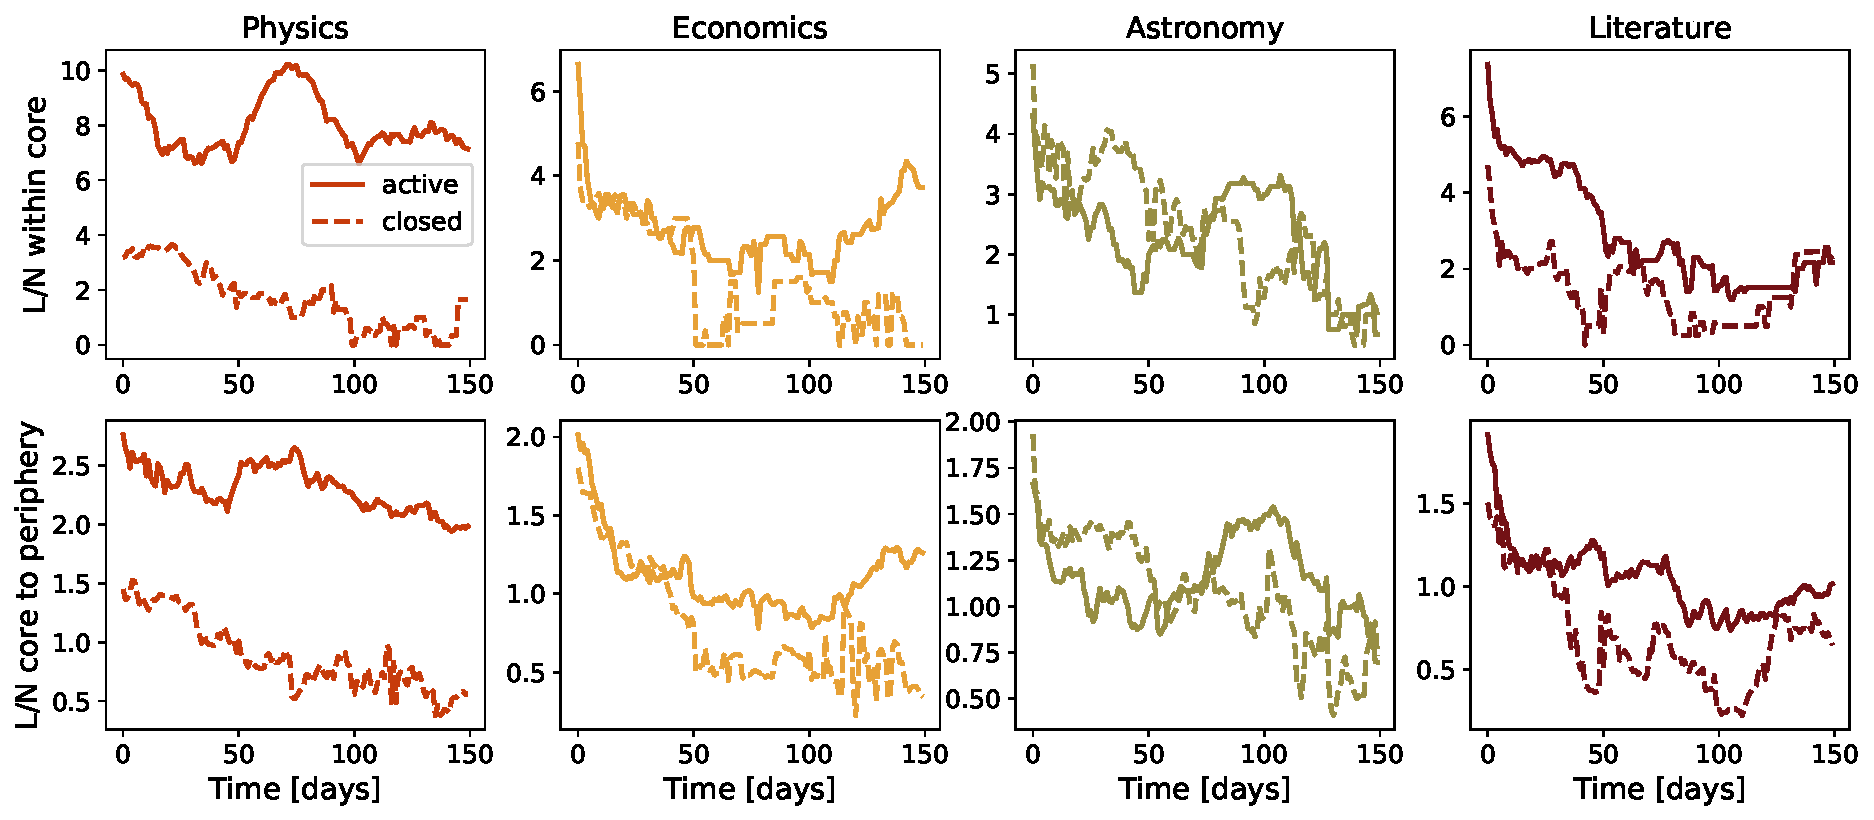
\includegraphics[width=\linewidth]{figures/stackexchange/core_connectivity.pdf}
	\caption{Links per node in core and links per node between core and periphery.}
	\label{fig:links_per_node}
\end{figure}


\subsection{Core-periphery structure of the interaction networks}


In Q-A communities are common two types of users: popular and casual users. Popular users tend to generate the majority of interactions - they are likely to post more questions, also take part in answering questions and tend to engage discussions through comments. For popular users we consider $10 $  of most active users. We analyse interactions between popular and casual users and  among popular users in the  sub-networks of 30 days [t+30). In both cases the number of links per nodes in active sites are larger than in closed communities (figure \ref{fig:pop_cas_users}).

Although this separation of users puts an emphasis on  differences between closed and active sites, it does not guarantee that all popular users are in the top 10 . To solve this dilemma we use the SBM (Stochastic Block Model) algorithm) to detect the core and the periphery of each 30 days sub-network. Such a split of users leads us to similar conclusions as before. (see figure \ref{fig:windows} - 2nd column)

Stochastic models start from random configuration and the algorithm  can converge to different local stable states. For each 30 days sub-network we run 50 iterations of SBM and choose the model parameters $\theta, p$ according to minimum description length. As example we show analysis of inferred sample of  core-periphery structures for 30 days area51 astronomy networks, Figure \ref{fig:sample}. We represent mean minimum description length (MDL) and mean number of nodes in the core with standard deviation. MDL does not change much among inferred core-periphery structures, still difference between obtained configurations is notable in the number of nodes in the core.  To investigate in more details similarity between obtained core-periphery configurations in the sample we calculate several measures between pair-wised partitions such as normalized mutual information, adjusted rand index, F1 measure and Jaccard index. Those measures are larger than 0.5, and in most cases higher than 0.9 indicating stability of the inferred core-periphery structures.
%TODO
%. MDL does not change much among infered core-periphery structure, Fig \ref{fig:sample} while looking into adjusted rand index we can notice that difference exists. Still, ARI between pair-wised compared partitions is large ($ari >0.9$) indicating stability of inferred structures.    



To study the stability of the core across the time we compute Jaccard’s coefficient between core users in [t+30) networks selected at times $t_1$ and $t_2$, (figure \ref{fig:jaccard_hm}). Higher values of the Jaccard index indicate that core users tend to stay in the core. The detected cores experience a lot of change over time and the highest overlap between core users is in the network closer in the time. The average Jaccard index between core users in all sub-networks separated by time interval $|t_1 - t_2|$ with standard deviation confidence interval is presented in figure \ref{fig:jaccard_mean}. Compared to closed sites, active sites show more stability in the core. Even the number of core users obtained in the launched and closed communities are comparable \ref{fig:core_size} (a high difference is found only for physics ), the ratio between total core and periphery reputation is evidently higher in the active than in closed sites, figure \ref{fig:dr_core_per}.  

\begin{figure}[h!]
	\centering
	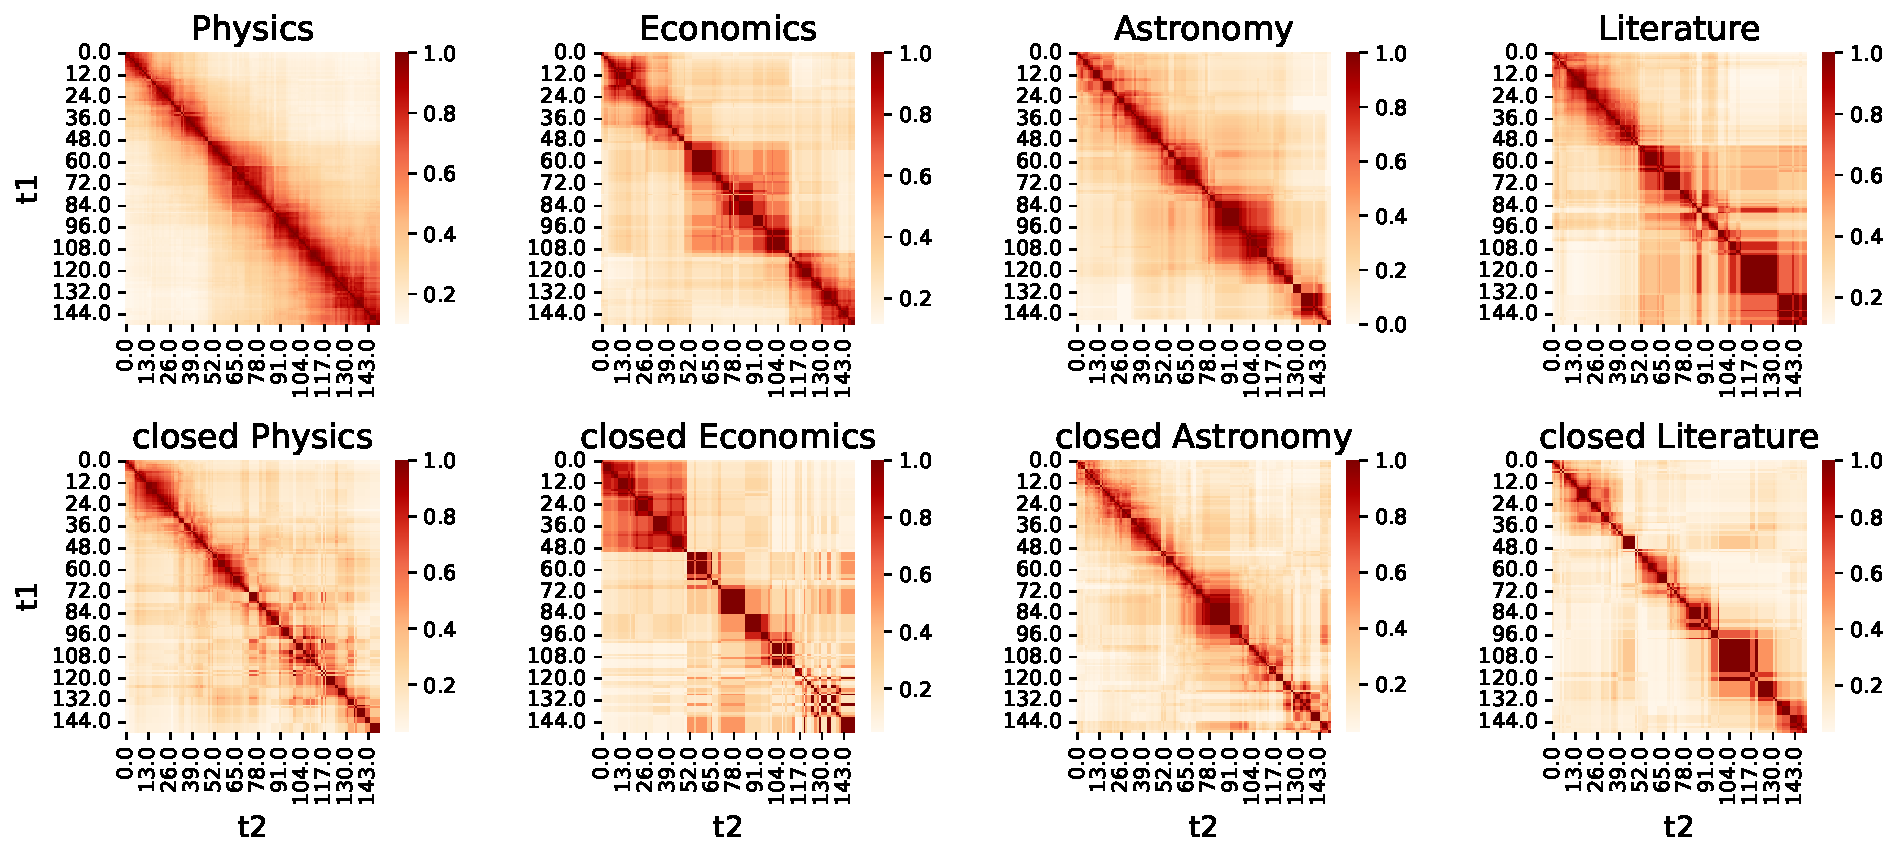
\includegraphics[width=\linewidth]{figures/stackexchange/jaccard_heatmap.pdf}
	\caption{Jaccard index between core users in  sub-networks at time points $t1$ and $t2$}
	\label{fig:jaccard_hm}
\end{figure}

\begin{figure}[h!]
	\centering
	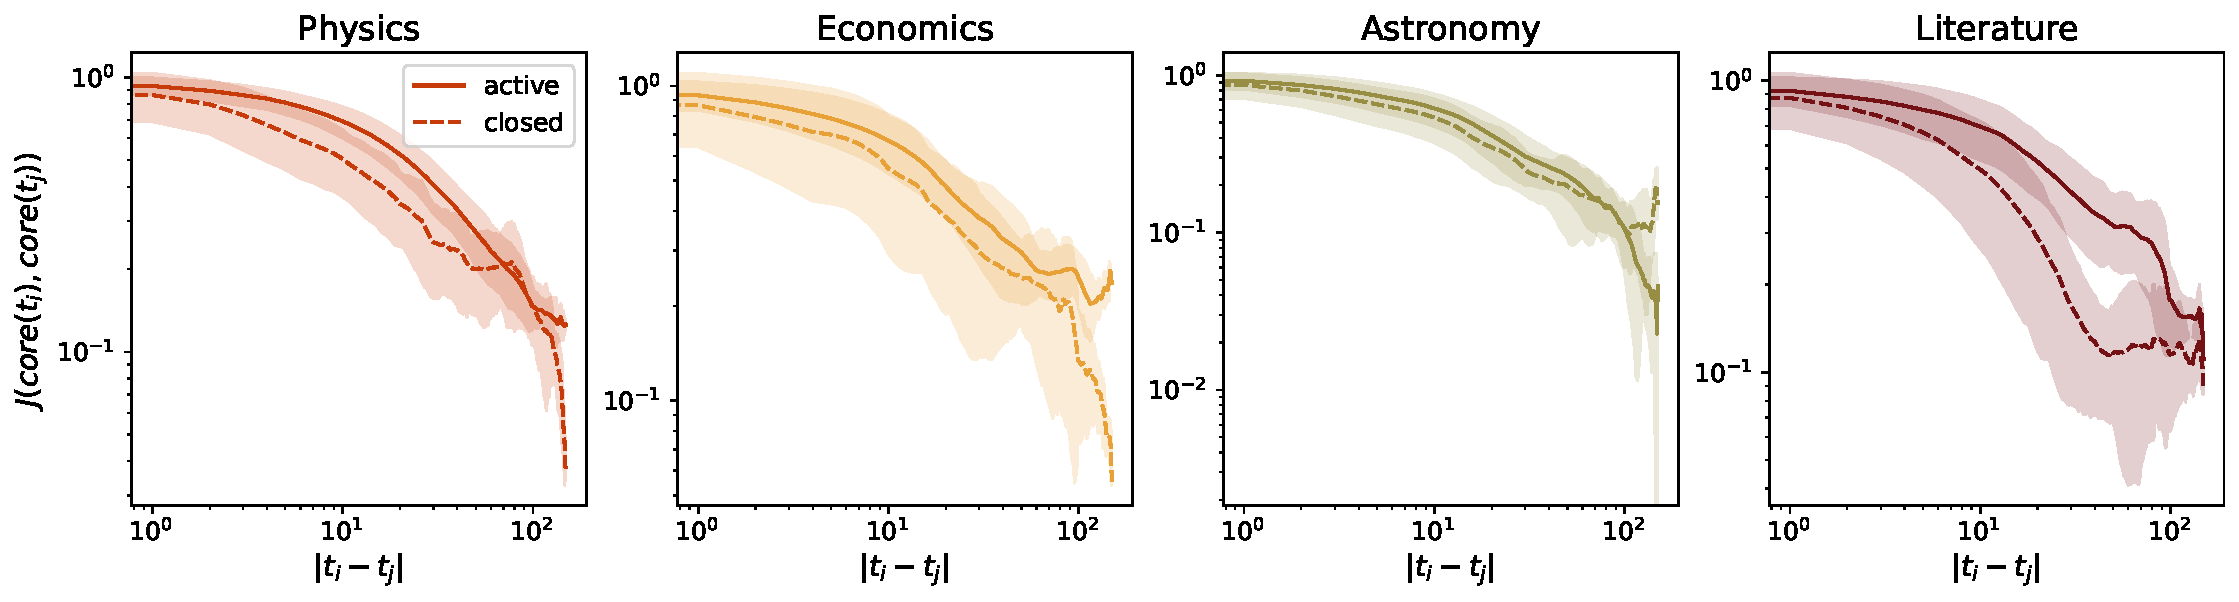
\includegraphics[width=\linewidth]{figures/stackexchange/jaccard.pdf}
	\caption{Jaccard index between core users in 30days sub-networks for all possible pairs of 30 days sub-networks separated by time interval $|t_i - t_j|$}
	\label{fig:jaccard_mean}
\end{figure}

% mozda bi ove dve slike core size i ration between reputations mogli da spojimo (slike A9 i A10), samo da se doda treci red na A9? 

\begin{figure}[h!]
	\centering
	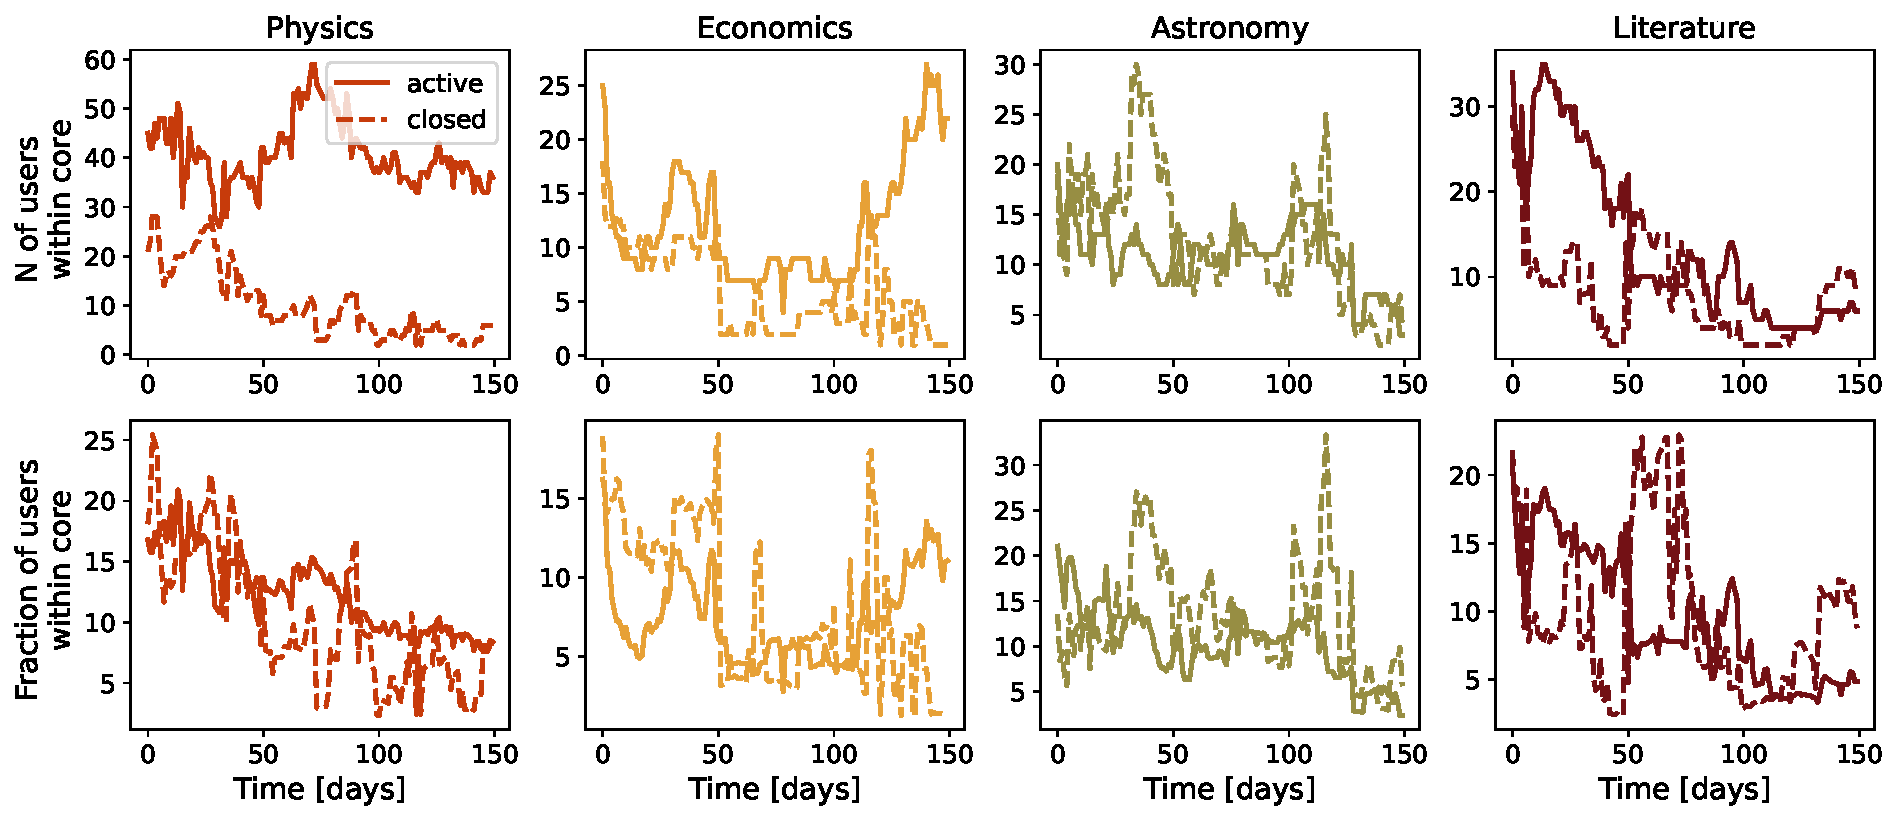
\includegraphics[width=\linewidth]{figures/stackexchange/core_users.pdf}
	\caption{Just for reference size of the core (top) and fraction of users in core (bottom). Solid lines - active sites; dashed lines - closed sites.}
	\label{fig:core_size}
\end{figure}

\begin{figure}[h!]
	\centering
	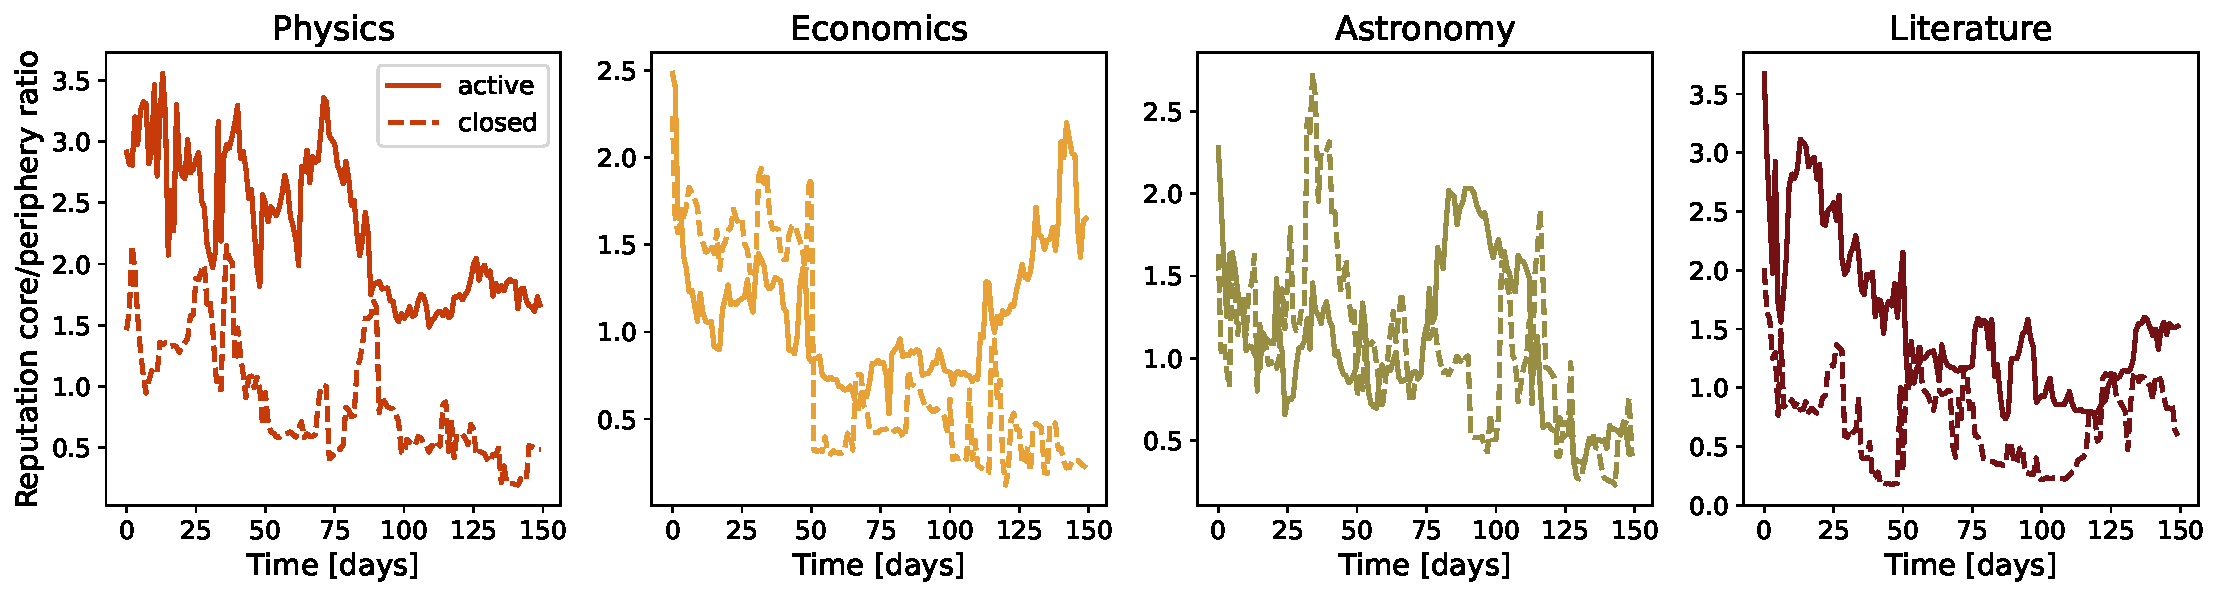
\includegraphics[width=\linewidth]{figures/stackexchange/core_per_ratio_reputation.pdf}
	\caption{Ratio between the total reputation within network core and periphery. Solid lines beta communities, dashed lines area 51 communities.}
	\label{fig:dr_core_per}
\end{figure}

\clearpage
\begin{figure}[h!]
	\centering
	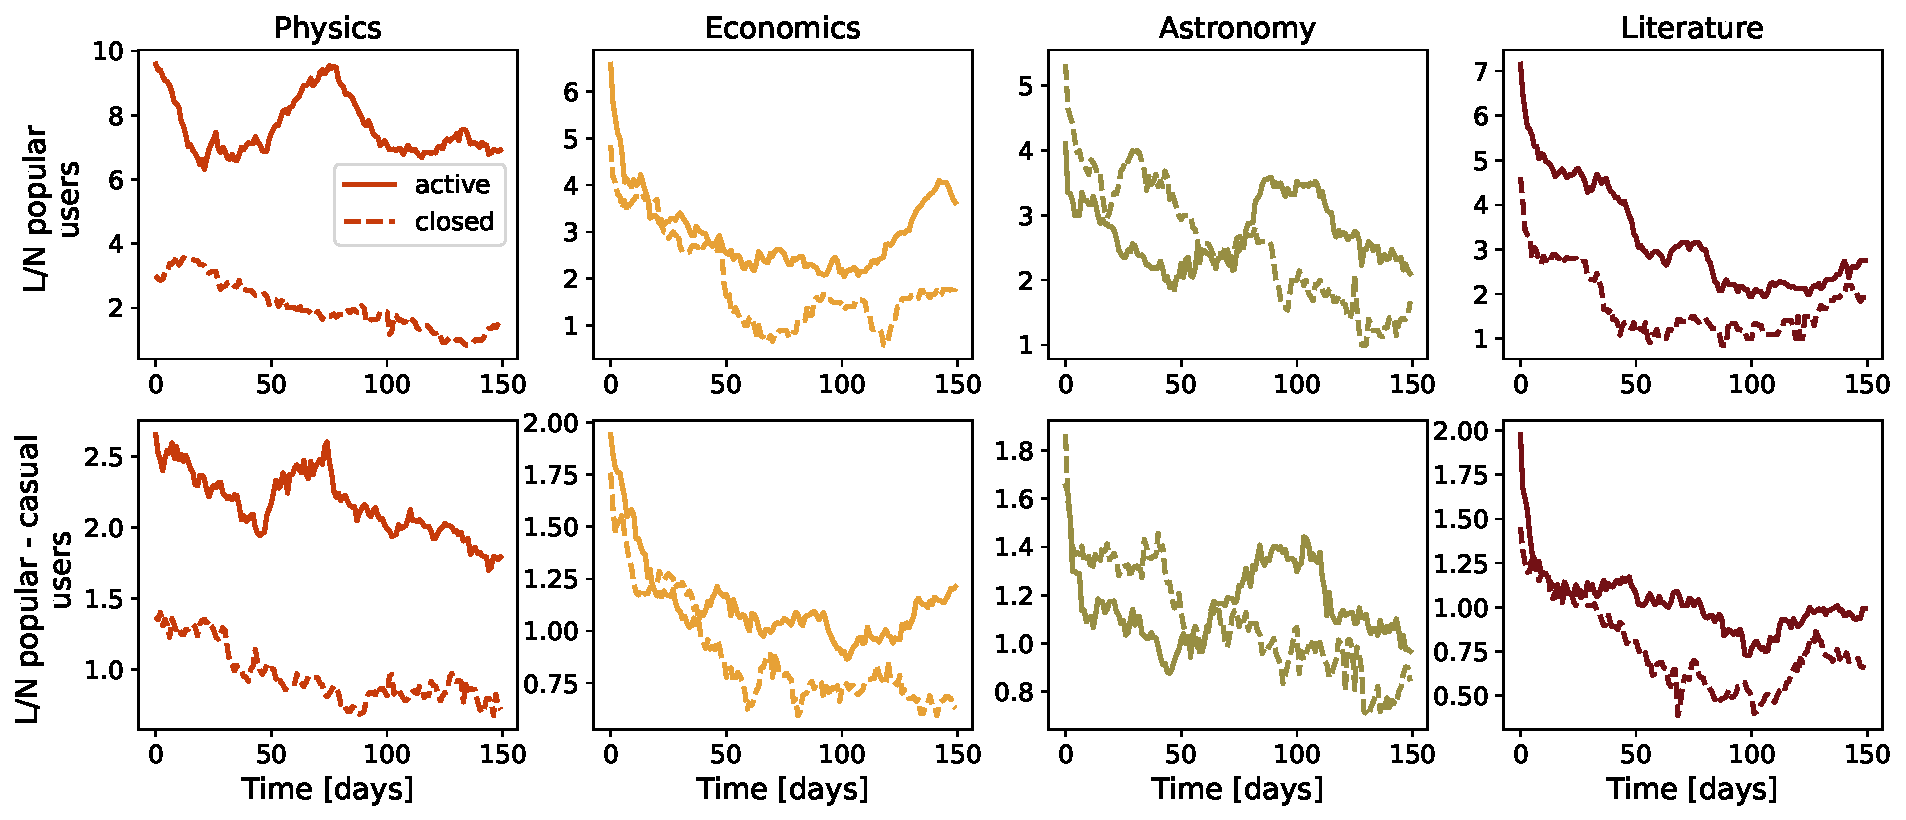
\includegraphics[width=\linewidth]{figures/stackexchange/popular_casual_users.pdf}
	\caption{Links per node among popular users (top 10\% of users) and between popular and casual users (everyone but popular users).
		Reminder: only 3rd and 5th columns should stay and only for reference to previous research, while our point is to this selection via core/periphery decomposition without thresholding.}
	\label{fig:pop_cas_users}
\end{figure}

